\documentclass[10pt, a4paper]{article} % 设置字体大小和纸张类型
\usepackage{fontspec}
\setmainfont{Times New Roman}

\usepackage{booktabs} % 支持更专业的表格线条
\usepackage{ctex}
\usepackage{caption} % 插图和表格的标题格式
\usepackage{amsmath, amsfonts, amssymb} % 数学公式支持
\usepackage{graphicx} % 插入图片
\usepackage{hyperref} % 超链接支持
\usepackage{geometry}
\usepackage{titlesec}
\usepackage{fmtcount} % 用于数字到中文的转换
\usepackage{enumitem} % 加载 enumitem 宏包
\usepackage{multirow} % 支持多行单元格
\usepackage{diagbox}
\usepackage{makecell} % 支持单元格内换行
\usepackage{tikz}
\usepackage{booktabs} % 支持更专业的表格线条
\usepackage{multirow} % 支持多行单元格
\usepackage{makecell}
\usepackage{unicode-math}
\setmathfont{Latin Modern Math}
\geometry{a4paper, margin=1.5cm} % 设置页边距

\renewcommand{\thesection}{\chinese{section}、}
\renewcommand{\thesubsection}{\arabic{subsection}.}


\begin{document}

\begin{titlepage}
    \newgeometry{left=0cm, right=0cm, top=0cm, bottom=0cm}
    \centering
    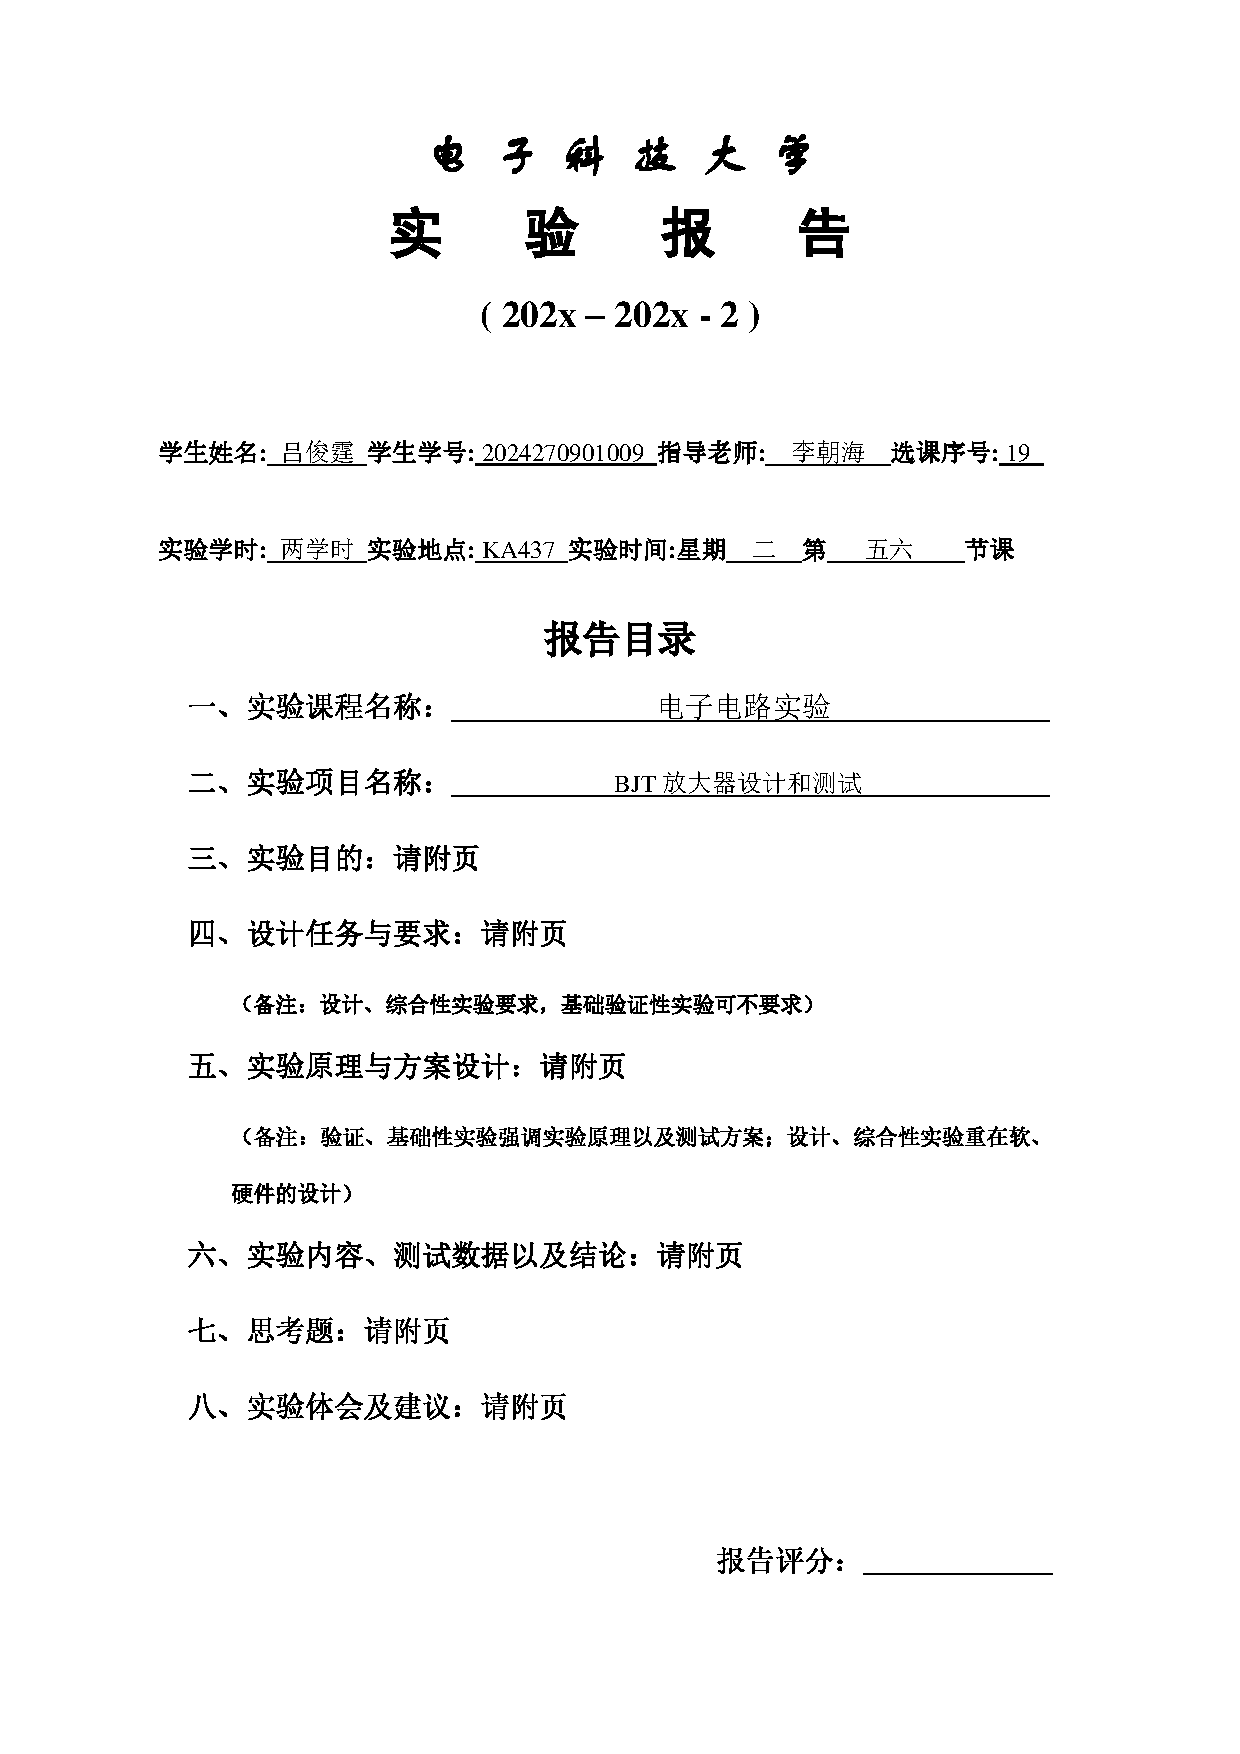
\includegraphics[page=1, width=0.9\textwidth, keepaspectratio]{image/实验报告撰写封面.pdf}
    \restoregeometry
\end{titlepage}

\setcounter{section}{2}

\section{实验目的}

\begin{enumerate}[leftmargin=50pt,label=(\arabic*)] % 设置序号格式为(1)
    \item 了解BJT的基本放大特性;
    \item 掌握BJT共射放大电路的分析与设计方法;
    \item 掌握放大电路静态工作点的测试方法;
    \item 掌握放大电路放大倍数(增益)的测试方法;
    \item 掌握放大电路输入、输出电阻的测试方法;
    \item 掌握放大电路幅频特性曲线的测试方法。
\end{enumerate}

\section{设计任务与要求}

暂不需要。

\section{实验原理与方案设计}
\subsection{实验原理}
使晶体管(BJT管)工作在放大状态的外部条件是发射结正向偏置且集电结反向偏置。因此对于NPN管工作在放大时, 三个电极的直流偏置电压关系应该满足$V_C > V_B > V_E$二对于PNP管工作在放大状态时, 三个电极的直流偏置电压关系应该满足$V_E > V_B > V_C$。

BJT管再应用中, 往往将一个电极作为输入端, 一个电极作为输出端, 第三个电极作为公共端, 即为将其作为伤口期间来使用, 有共射、共基和共集接法。
    
(1) 共射极放大器原理

共射放大器时晶体管放大电路中常用的一种基本放大电路, 它能把频率几十赫兹到几百千赫的信号进行不失真放大。采用基极分压射极偏置电路的公社放大器的电路原理图如下, 对应直流通路如图。

\begin{figure}[ht]
    \centering 
    \begin{minipage}{0.54\linewidth}
        \centering
        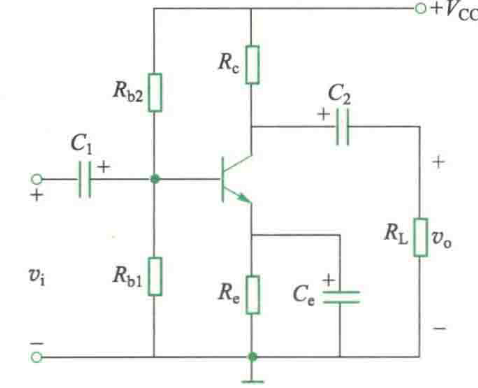
\includegraphics[width=\linewidth]{image/1.png}
        \caption{图为电路原理图}
    \end{minipage}
    \hfill
    \begin{minipage}{0.34\linewidth}
        \centering
        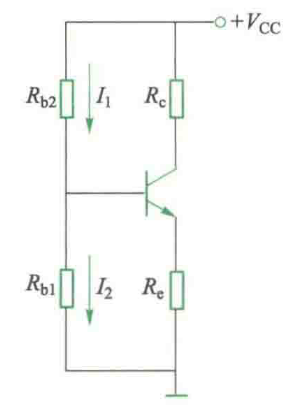
\includegraphics[width=\linewidth]{image/2.png}
        \caption{图为直流通路}
    \end{minipage}
    % Ensure all environments are properly closed
\end{figure}

此偏置电路称为基极分压射极偏置电路, 是一种可以稳定工作点的电路。当该电路满足 $I_1$、$I_2$ 远大于 $I_B$ 时, 基极偏置电压 $V_B$ 只由 $V_{CC}$、$R_1$ 和 $R_2$ 决定, 与 BJT 参数无关。由于 $V_{CC}$、$R_1$ 和 $R_2$ 对温度均不敏感, 所以 $V_B$ 稳定。当某种原因(如温度增加、电源电压增加或更换 $h_{FE}$ 更大的 BJT)使得静态工作点 $I_C$ 增加时, 电路依靠直流负反馈的作用, 可以抑制 $I_C$ 的增加, 使得静态工作点稳定。

\newpage
分析放大电路时, 可以用直流通路求解静态工作点, 交流通路求解放大器的性能指标。

直流通路:当放大器未加输入信号($v_i = 0$), 即电路处于静态时, 直流电流流经的电路称为放大器的直流通路。直流通路其实就是建立放大器工作点的电路。画直流通路时应将电容开路、电感短路。

交流通路:信号输入放大器以后, 晶体管和一些元件上的电流电压会在直流电流电压上叠加交流电流电压分量(即信号成分), 故可以画出一个只反映放大器交流电流和交流电压之间关系的电路, 这称为交流通路或交流电路。画交流通路时, 恒压源、耦合电容以及旁路电容应该短路, 而恒流源以及高频扼流圈应该开路。


(1.1)工作点估算


直流通路中, 因为 $I_1$ 和 $I_2$ 远大于 $I_B$, 即可忽略 $I_B$, 则 $I_1 = I_2$, 由 $R_1$ 和 $R_2$ 分压可知静态工作点基极电压 $V_{BQ}$ 为

 $$
V_{BQ} \approx \frac{R_2}{R_1 + R_2} V_{CC}
$$ 

又由于发射结正向偏置, 可知基极电压与发射极之间电压差为 PN 结的正向电压 $V_{BE}$, 对于硅管 $V_{BE} \approx 0.7 \text{ V}$, 可求得

$$
I_{EQ} = \frac{V_{BQ} - V_{BE}}{R_e}
$$ 
工程估算时有, $I_{CQ} \approx I_{EQ}$, 故有

$$
V_{CEQ} \approx V_{CC} - (R_c + R_e) I_{CQ}
$$ 

(1.2)交流指标的计算
图 1放大电路的交流小信号等效电路如图3 所示, 由交流小信号等效电路可以计算该共射放大器的交流指标。

\begin{center}
\begin{figure}[ht]
    \centering
    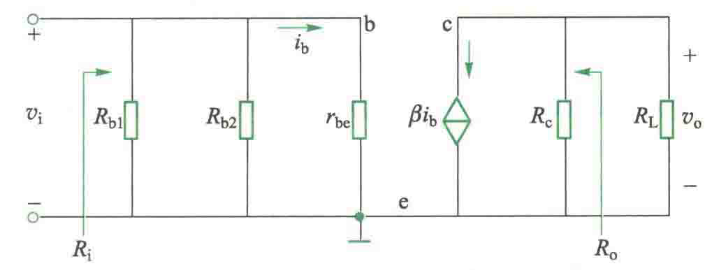
\includegraphics[width=0.8\textwidth]{image/3.png} % 请替换为实际的电路图文件名
    \caption{放大电路交流小信号等效电路}
    \label{fig:small_signal}
\end{figure}
\end{center}

电压增益 $A_v$ 为

$$
A_v = \frac{v_o}{v_i} \approx -\frac{\beta (R_C // R_L)}{r_{be}}
$$ 

输入电阻 $R_i$ 为

$$
R_i = R_1 // R_2 // r_{be}
$$ 

其中, be 间的等效电阻为 $r_{be} = r_{bb'} + (1 + \beta) \frac{V_T}{I_{EQ}}$, 室温(约为 27 ℃)时, $V_T \approx 26 \text{ mV}$。$r_{bb'}$ 为基区体电阻, 对于小功率管, 多在几十欧到几百欧, 估算时常取 200 Ω 左右。输出电阻 $R_o$ 为

$$
R_o \approx R_c
$$ 

(1.3)动态范围分析
动态范围分析即放大器线性工作时最大输出电压分析, 当输入信号的振幅不断增大时, BJT 会进入截止区或饱和区。BJT 不会进入截止区或饱和区的最大输出电压即放大器的动态范围可以在输出特性曲线上借助负载线来分析。

(2)电路设计要点

(2.1)设置放大器的静态工作点并计算、确定电阻元件的参数

发射结正偏, 极电结反偏是晶体管构成放大电路的前提条件, 因此必须首先设置好电路的直流工作状态, 即静态工作点 $Q$。在设计小信号放大电路时, 一般取 $I_C = 0.5 \sim 2 \text{ mA}$, 将 $Q$ 点设置在交流负载线的中间位置可使放大器具有最大动态范围。实际工作中, 也经常将 $Q$ 点设置在直流负载线的中点来近似, 即取 $V_{CEQ} = 0.5 V_{CC}$。根据 $V_{CEQ} \approx V_{CC} - (R_C + R_E) I_{CQ}$ 初步确定 $R_C$ 及电路其他参数后, 再根据动态性能指标的要求, 对 $Q$ 点进行一些调整。


(2.2)交流性能指标的约束

由于共射放大器输出电阻的公式为: $ R_o \approx R_c $ , 所以  $ R_c $  的值受到  $ R_o $  的限制, 一般  $ R_c $  要比  $ R_o $  稍微小一些。

又根据增益公式: $ A_v \approx \frac{-\beta (R_c // R_L)}{r_{be}} $ ,  $ R_c $  还要根据电路的增益  $ A_v $  进行调整, 以满足设计的各项动态性能指标。

(2.3)根据设计要求的下限频率  $ f_L $ , 确定电路中的耦合电容及旁路电容的参数

实际的放大器由于存在电抗元件, 从而使增益成为与频率相关的复数。其模与频率的函数关系称为放大器的幅频特性。当输入信号幅度保持不变时, 信号频率过低或过高, 输出幅度都会下降, 只在中间频率范围内, 输出幅度基本不变。

对于阻容耦合共射极放大器来说, 低频特性主要取决于容量较大的  $ C_1 $ 、 $ C_2 $  及  $ C_e $ , 高频特性主要取决于容量较小的晶体管 PN 结电容、负载电容及布线搭建时的杂散电容。

如果严格按照模拟电路理论来计算电容  $ C_1 $ 、 $ C_2 $  及  $ C_e $  同时存在时对放大器低频特性  $ f_L $  的影响, 是较为复杂的。在工程设计中, 为了简化计算, 通常以每个电容单独存在时的转折频率为基本频率, 再降低若干倍作为下限频率, 通常取  $ C_1 = C_2 $ 。本次设计不要求电容的约束, 搭建电路时, 电容可选 100  $\mu F$  左右的电解电容。

(3) 放大电路测试方法

(3.1)放大电路静态工作点的测试
静态工作点的测试实际就是直流电压、电流的测量。对直流电压的测量, 可以用数字万用表或示波器来进行测量。

对射极电流的测量可采用间接测试方法, 即测试出射极电阻两端的直流电压, 再除以射极电阻可得到射极静态电流。

(3.2)放大电路交流指标的测试
放大电路交流指标, 如电压增益、输入电阻、输出电阻以及通频带等, 常用输入正弦交流信号的方法进行间接测量。图 4 为放大器通用模型, 这里以放大器通用模型来说明这些指标的测试方法。

\begin{figure}[ht]
    \centering
    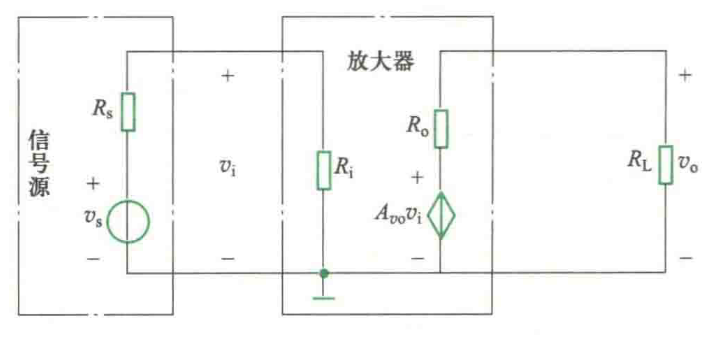
\includegraphics[width=0.8\textwidth]{image/4.png}
    \caption{放大器通用模型}
    \label{fig:amplifier_model}
\end{figure}

\subsection*{A. 电压增益的测试}
电压增益的测试比较简单, 工作点设定正确以后, 用信号源输出一个中频正弦小信号作为放大器的输入信号, 然后用交流毫伏表或者示波器直接测量放大器的输入信号电压有效值  $ V_i $  和输出信号电压有效值  $ V_o $ , 由  $ A_v = V_o / V_i $  即可得到。

\subsection*{B. 输入电阻的测试}
输入电阻是从放大器的输入口视入放大器的等效交流电阻。输入电阻要向信号源吸收信号功率, 因此, 输入电阻是在放大器输入口的信号源负载, 如图 5.6.4 所示的等效电阻  $ R_i $ 。输入电阻  $ R_i $  远大于信号源的内阻  $ R_s $  时, 放大器向信号源索取的功率就小, 对信号源的电压利用率就高。

当被测电路的输入电阻不太高时, 可以采用如图 5所示的“两次电压法”的方法进行测量。在信号发生器与放大器的输入端之间串接入一个已知电阻  $ R $ (称为取样电阻), 用交流电压表分别测出取样电阻  $ R $  两端对地的信号电压  $ V'_s $  和  $ V_i $  的值, 则可由下式计算出输入电阻  $ R_i $  的值:


 $$
R_i = \frac{V_i}{V'_s - V_i} = \frac{V_i}{V'_s - V_i} R
$$ 

注意:取样电阻  $ R $  的选择应与  $ R_i $  为同一数量级, 过小或过大都会使测量误差增大。

\begin{figure}[h]
    \centering
    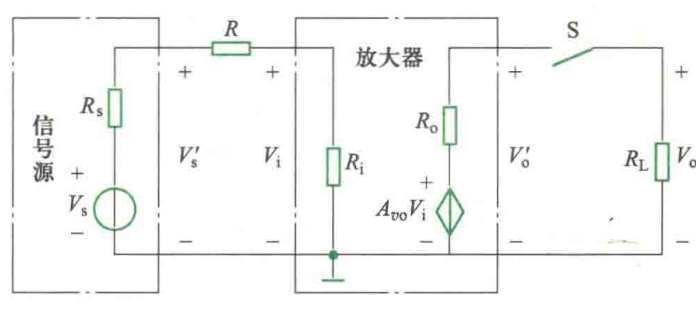
\includegraphics[width=0.8\textwidth]{image/5.png}
    \caption{阻抗测量原理图}
    \label{fig:input_resistance_measurement}
\end{figure}


\section*{C. 输出电阻的测量}

放大器要向负载提供信号功率, 因此, 放大器在输出口对负载而言, 等效一个新的信号源, 该信号源的内阻就是输出电阻, 如图 4 所示的等效电阻  $ R_o $ 。输出电阻是衡量放大器驱动负载能力大小的一个指标, 输出电阻  $ R_o $  越小, 则放大器驱动负载的能力就越高。

输出电阻仍然采用间接测量的“两次电压法”测量, 测量原理如图 5 所示。根据戴维南定理, 放大器的输出端口可等效为一个电压源与一内阻的串联, 等效电压源  $ V'_o $  即为空载( $ R_L = \infty $ )时的输出电压, 等效内阻  $ R_o $  即为放大器的输出电阻。因此, 分别测出放大器空载(开关 S 断开)时的输出电压  $ V'_o $  和接入负载时的输出电压  $ V_o $ , 即可计算出输出电阻的值


 $$
R_o = \frac{V'_o - V_o}{\frac{V_o}{R_L}} = \left(\frac{V'_o}{V_o} - 1\right) R_L
$$ 

注意: $ R_L $  接入前后, 要保证输入信号的大小不变。


\section*{D. 幅频特性测量}

获取二端网络幅频特性曲线可以采用点频法(逐点法), 即保持输入信号大小不变, 改变输入信号的频率, 测量对应的输出电压值, 即可绘制幅频特性曲线。在测试过程中通常用毫伏表或示波器监测输入信号, 并保持输入信号不变, 如果改变频率后输入信号有所变化, 必须调节信号发生器使输入信号维持原来的大小。

\newpage


\section{实验内容、测试数据以及结论}
\subsection{实验内容}

用给定的晶体管 2SC1008 设计具有最大动态范围的共射放大器, 晶体管参数为  $ r_{bb} = 200 \, \Omega $ 、 $ \beta = 200 \sim 300 $ (可用具有相关功能的数字万用表实测晶体管的  $ \beta $  值)。已知  $ V_{CC} = 12 \, \text{V} $ , 设计要求: $ I_C = 1.5 \sim 2.0 \, \text{mA} $ 、 $ R_i > 1.5 \, \text{k}\Omega $ 、 $ R_o < 2.5 \, \text{k}\Omega $ 、 $ A_v > 50 $ 。在面包板上搭建所设计电路, 并完成下列测试。

\subsubsection{静态工作点调整与测试}

令  $ V_{CC} = +12 \, \text{V} $ , 用数字万用表测量  $ V_E $ 、 $ V_B $ 、 $ V_C $ , 计算  $ V_{BE} $ 、 $ I_{EQ} $ 、 $ V_{CE} $ , 数据记入表 1 中。

\begin{table}[ht]
    \centering
    \caption{静态工作点的测量}
    \begin{tabular}{c|c|c|c|c|c}
        \toprule
         $ V_E $  &  $ V_B $  &  $ V_C $  &  $ V_{BE} $  &  $ I_{EQ} $  &  $ V_{CE} $  \\
        \midrule
        2.25V&2.89V&7.36V&0.65V&2.25mA&5.11V\\
        \bottomrule
    \end{tabular}
\end{table}

\subsubsection{放大倍数的测试}

用函数发生器输出一个正弦波信号作为放大器的输入信号, 设置信号频率  $ f = 1 \, \text{kHz} $ ,  $ V_i = 5 \, \text{mV} $ , 测量  $ V_o $ , 计算放大器的电压放大倍数(增益) $ A_v $ 。数据填入表 2 中。

\begin{table}[ht]
    \centering
    \caption{放大倍数的测量}
    \begin{tabular}{c|c|c|c|c}
        \toprule
        测试条件 & 工作状态 & 输出电压 ( $ V_o $ ) & 放大倍数 ( $ A_v $ ) & 输出波形 \\
        \midrule
         $ f = 1 \, \text{kHz} $  & 正常 &780mV&156&正弦波\\
         $ V_i = 5 \, \text{mV} $  & & & & \\
        \bottomrule
    \end{tabular}
\end{table}

\subsubsection{放大器输入电阻的测量}

在放大器输入口串接一个取样电阻  $ R $ , 用“两次电压法”测量该放大器的输入电阻  $ R_i $ , 数据填入表 3 中。

\begin{table}[ht]
    \centering
    \caption{输入电阻的测量}
    \begin{tabular}{c|c|c|c|c}
        \toprule
         $ V'_s $  &  $ V_i $  & 取样电阻  $ R $  &  $ R_i $  \\
        \midrule
        20mV&1.5mV&30K&2.4K\\
        \bottomrule
    \end{tabular}
\end{table}



\section*{放大器输出电阻的测量}

在放大器输出口选择一个合适的负载电阻  $ R_L $ , 运用“两次电压法”分别测量空载与接上负载时的输出电压值  $ V'_o $  和  $ V_o $ , 数据填入表 4 中。

\begin{table}[ht]
    \centering
    \caption{输出电阻的测量}
    \begin{tabular}{cccc}
        \toprule
         $ V'_o $  &  $ V_o $  & 负载电阻  $ R_L $  &$R_o$\\
        \midrule
        1.55V&0.8V&2K&1.825K\\
        \bottomrule
    \end{tabular}
\end{table}
\newpage
\section*{放大器频率特性的测量}

用点频测试法测量放大器空载时的频率特性, 并求出带宽。测试数据填入表 5 中, 并绘出幅频特性曲线。

\begin{table}[ht]
    \centering
    \caption{幅频特性的测试}
    \begin{tabular}{cccccccccc}
        \toprule
        频率值/Hz &  $ f_l $  &  $ f_0 $  &  $ f_H $  & 带宽  $ \Delta f $  \\
        \midrule
        &145&1k&272K& \\
         $ V'_o/V $ &0.56V&0.8V&0.56V&272K\\
        \bottomrule
    \end{tabular}
\end{table}




\subsection{实验结论}

1.输入信号的频率大小会影响放大器的放大倍数, 且在一定范围内的频率可以使放大器的放大倍数稳定在一个较高的水平。

2 实验前应估算好输入电阻、输出电阻的大小, 电阻阻值的选择会影响放大器放大的效果。

\section{思考题}
\subsection{题面}
\begin{enumerate}[leftmargin=50pt,label=(\arabic*)] % 设置序号格式为(1)
    \item 在BJT放大电路中, 直流电源的作用是什么? 如何设定放大器的静态工作点? 
    \item 影响放大器增益的主要因素有哪些? 
    \item 放大器输入电阻、输出电阻的物理意义是什么? 

\end{enumerate}
\subsection{回答}

\begin{enumerate}[leftmargin=50pt,label=(\arabic*)] % 设置序号格式为(1)
    \item 直流电源的作用是建立合适的静态工作点, 使得晶体管进入放大状态, 保证发射结正向偏置,集电结反向偏置还要使放大器能在正常放大的时候不会产生非线性失真。静态工作点一般选在适中的IC, 选小了容易出现小信号失真, 选大会出现饱和失真。
    \item 影响放大器增益的主要因素有晶体管的本身参数(如β、hfe等)、负载电阻、交流信号源内阻、偏置网络对信号的分压作用等。
    \item 放大器输入电阻是指在放大器输入端加上一个交流信号源时, 信号源看到的等效电阻。它反映了放大器对信号源的负载程度, 越大越好。输出电阻是指在放大器输出端接上一个负载时, 负载看到的等效电阻。它反映了放大器对负载的匹配程度, 越小越好。
\end{enumerate}

\section{实验体会及建议}
\subsection{实验体会}
测量时应注意小心调试仪器, 尽量将读数稳定在误差允许范围内进行读数。
\subsection{建议}
注意仪器正负极的接入, 防止反接造成仪器损坏。


\end{document}
